\documentclass{article}
\usepackage[table]{xcolor}
\usepackage[T1]{fontenc}
\usepackage{tgschola}
\usepackage[a4paper, total={6in, 8in}, margin=2cm]{geometry}
\usepackage{lipsum}
\usepackage{fancyhdr}
\usepackage{lastpage}
\setlength{\headheight}{48.2pt}
\usepackage{boxedminipage}
\usepackage{graphicx}
\usepackage{tikz}
\usetikzlibrary{shapes.geometric}
\usepackage{wrapfig}
\usepackage{float}
\usepackage{subfig}
\usepackage{circuitikz}
\usetikzlibrary{arrows}
\usepackage[T1]{fontenc}
\usepackage{tgbonum}
\usepackage[most]{tcolorbox}
\usepackage{textgreek}
\usepackage{graphicx}
\graphicspath{ {./} }
\usepackage[T1]{fontenc}
\usepackage{multicol}
\usepackage{siunitx}
\sisetup{output-decimal-marker = {,}} %para que use coma en vez de punto
\usepackage[usestackEOL]{stackengine}
\graphicspath{ {./imagenes/} }
\pagestyle{fancy}
\usepackage{enumitem}
\usepackage[most]{tcolorbox}
\usepackage[option ]{askmaps}
\usepackage{circuitikz}
\usepackage{float}
\usepackage{adjustbox}
\usepackage{amsmath}
\usepackage{array}
\usepackage{multirow}
\usepackage{geometry}
\usepackage{booktabs}
\usepackage{tikz-timing}
\usepackage{url}
\usepackage{tabularx}
\usepackage{geometry}
\usepackage{changepage}
\usepackage[implicit=false]{hyperref}

\definecolor{headergray}{RGB}{220,220,220}


%%Modificar los siguientes valores segun la materia/tp
\newcommand{\Titulo}{Trabajo Práctico 1.1}
\newcommand{\Subtitulo}{Electricidad y circuitos en C.C.}
\newcommand{\Version}{Versión 261C.01}
\newcommand{\Carrera}{INGENIERÍA EN INFORMÁTICA}
\newcommand{\Asignatura}{3631 - Fundamentos de sistemas embebidos}
\newcommand{\Tema}{Electricidad y circuitos en C.C.}
\newcommand{\Unidad}{1.1}
\newcommand{\Objetivo}{Comprender las magnitudes físicas elementales de la electricidad, tensión, corriente y resistencia. Conocer los componentes comunes que forman los circuitos en corriente continua. Ser capaz de entender y analizar circuitos simples}
\newcommand{\TiempoResolucion}{1 semana}
\newcommand{\Metodologia}{Ejercicios verificados en simuladores}
\newcommand{\Entrega}{No obligatoria}


\fancyhead[L]{\framebox(128,64){\includegraphics[scale=0.18]{diit}}}
\fancyhead[C]{\framebox(224,64){\Longstack{\textbf{\Titulo}\\\textbf{\Subtitulo}\\Pág. \thepage\ de \pageref{LastPage}}}}
\fancyhead[R]{\framebox(128,64){\includegraphics[scale=0.055]{logo}}}
\renewcommand{\headrulewidth}{0.0pt}
\renewcommand{\footrulewidth}{0pt}



\begin{document}
	
		\centering\LARGE{\textbf{\Version}}
	\large
	\\
	\begin{center}
		\begin{tabular}{|p{16cm}|} % 'l' for left-aligned, 'p' for paragraph with specified width
			
			\hline
			\rule{0pt}{15pt}
			\textbf{Carrera: \Carrera} \\
			\hline
			\rule{0pt}{15pt}
			\textbf{Asignatura:}  \Asignatura \\
			\hline
			\rule{0pt}{15pt}
			\textbf{Tema:}  \Tema \\
			\hline
			\rule{0pt}{15pt}
			\textbf{Unidad:}  \Unidad \\
			\hline
			\rule{0pt}{15pt}
			\textbf{Objetivo:} \Objetivo \\
			\hline
			\rule{0pt}{15pt}
			\textbf{Competencias a desarrollar:} 
			\begin{itemize}
				\item Concepción, diseño y desarrollo de proyectos de ingeniería en informática.
				\item Gestión, planificación, ejecución y control de proyectos de ingeniería en informática.
				\item Utilización de técnicas y herramientas de aplicación en la ingeniería en informática.
				\item Generación de desarrollos tecnológicos y/o innovaciones tecnológicas.
				\item Desarrollo de una actitud profesional emprendedora.
				\item Aprendizaje continuo
				\item Actuación profesional ética y responsable.
				\item Comunicación efectiva.
				\item Desempeño en equipos de trabajo.
				\item Identificación, formulación y resolución de problemas de ingeniería en informática
			\end{itemize} \\
			\hline
			\rule{0pt}{15pt}
			\textbf{Descripción de la actividad:} 
			\begin{enumerate}
				\item  Tiempo estimado de resolución: \TiempoResolucion
				\item Metodología: \Metodologia
				\item Forma de entrega: \Entrega
				\item Metodología de corrección y feedback al alumno: Presencial y por Miel.
			\end{enumerate} \\
			\hline
		\end{tabular}
	\end{center}
	
	\clearpage
	
	
	%% Hacer que las tablas tengan un poco de padding
	\def\arraystretch{1.2}
	
	\section*{A- Electricidad y Circuitos en Corriente Continua}
	\begin{enumerate}[label=\textbf{A.\arabic*}]
		\item Explique cuales son los elementos que conforman el átomo\\
		\begin{center}
		\includegraphics[scale=0.2]{atomo}
		\end{center}
		\item Dados los siguientes casos para electrones y protones, indique si se produce atracción o repulsión.\\
			\begin{enumerate}
				\item
				\begin{center}
					\begin{tikzpicture}
						\draw (0,0) circle [radius=0.3] node {$+$};
						\draw (2,0) circle [radius=0.3] node {$-$};
					\end{tikzpicture}
				\end{center}
				\item
				\begin{center}
					\begin{tikzpicture}
						\draw (0,0) circle [radius=0.3] node {$+$};
						\draw (2,0) circle [radius=0.3] node {$+$};
					\end{tikzpicture}
				\end{center}
				\item
				\begin{center}
					\begin{tikzpicture}
						\draw (0,0) circle [radius=0.3] node {$-$};
						\draw (2,0) circle [radius=0.3] node {$-$};
					\end{tikzpicture}
				\end{center}
			\end{enumerate}
		
		\item Explique cuáles son las unidades de medida para:
			\begin{itemize}
				\item Tensión
				\item Corriente
				\item Resistencia
				\item Carga Eléctrica
			\end{itemize}
		\item Encuentre la resistividad $(\Omega . m)$  de los siguientes materiales y ordene los mismos en forma ascendente indicando primero el mejor conductor. 
		\begin{multicols}{3}
		\begin{itemize}
			\item Madera
			\item Plata
			\item Vidrio
			\item Teflón
			\item Oro
			\item Cobre
			\item Acero
			\item Aluminio
			\item Aire
		\end{itemize}
	\end{multicols}
	   \item Utilizando la ley de Ohm $(V = I . R)$ despeje los valores de R y de I, luego complete el triangulo mnemotécnico\\
	   \begin{minipage}{.45\textwidth}
	   \begin{itemize}
	   	\item $I=$
	   	\item $R=$
	   \end{itemize}
   		\end{minipage}
   	\begin{minipage}{.55\textwidth}
	  
	   	\begin{tikzpicture}
	   		\node[isosceles triangle,
	   		draw,
	   		rotate=90,
	   		fill=white,
	   		minimum size =1.5cm] (T1)at (0,0){};
	   		\draw[rotate=90] (0.3,0.4) -- (0.3,-0.4);
	   		\draw (00,0.3) -- (00,-0.5);
	   	\end{tikzpicture}
	\end{minipage}
	 \item 
	   Complete las siguientes tablas basadas en el código de colores de las resistencias
	   Use una calculadora de resistencias como: https://www.digikey.com/es\\/resources/conversion-calculators/conversion-calculator-resistor-color-code o \\ https://tools.mlista.uno/electronica/codigo-de-color-de-resistencia
	   \\
	    
	   %\begin{table}[h]
	   	
	   	%\centering
	   	\begin{tabular}{|c|c|c|c|c|c|}
	   		\hline
	   		\rowcolor{headergray}
	   		{Primera}& 	{Segunda} & 	{Cant. ceros} & 	{Tolerancia}  & 	{Valor }$\mathbf{\Omega }$& 	{\% Tolerancia} \\ \hline
	   		Marrón& Naranja& Violeta & Dorado  & $\SI{130}{\mega\ohm}$ & 5\% \\ \hline
	   		Rojo& Rojo & Rojo   &Plateado  &  &  \\ \hline
	   		Violeta &Blanco  &Naranja  &Plateado  &  &  \\ \hline
	   		Amarillo&Azul  &Marrón  &Dorado  &  &  \\ \hline
	   		Verde&Azul  &Negro  &Plateado &  &  \\ \hline
	   		Naranja&Marrón  &Amarillo  &Plateado  &  &  \\ \hline
	   		Blanco&Verde  &Dorado  &Plateado  &  &  \\ \hline
	   	\end{tabular}
	   %\end{table}
   
    %\begin{table}[h]
    	%\centering
   	\begin{tabular}{|c|c|c|c|c|c|}
   		\hline
   		\rowcolor{headergray}
   		{Primera}& 	{Segunda} & 	{Cant. ceros} & 	{Tolerancia}  & 	{Valor }$\mathbf{\Omega }$& 	{\% Tolerancia} \\ \hline
   		Marrón&Verde&Naranja&Dorado&$\SI{15}{\kilo\ohm}$&5\%\\ \hline
   		&&&&$\SI{300}{\ohm}$& 10\% \\ \hline
   		&&&&$\SI{570}{\ohm}$&5\% \\ \hline
   		&&&&$\SI{1,2}{\kilo\ohm}$&10\% \\ \hline
   		&&&&$\SI{3,3}{\kilo\ohm}$&10\% \\ \hline
   		&&&&$\SI{2}{\mega\ohm}$&5\%  \\ \hline
   		&&&&$\SI{1,5}{\kilo\ohm}$&10\%  \\ \hline
   	\end{tabular}
   %\end{table}
	\par
	\item Defina qué se entiende por sentido de circulación de corriente real y convencional.\\
	 
	
	\begin{minipage}{.55\textwidth} 
	\item
	Indique con una flecha el sentido de circulación \textbf{real} en el siguiente circuito (ireal) y luego con otra flecha el sentido de circulación \textbf{convencional} (iconv) \label{aohm}
	\end{minipage}
	\begin{minipage}{.25\textwidth}
	\begin{tikzpicture}
		% Paths, nodes and wires:
		\draw (6.75, 7.25) to[battery1, l_={$V1$}, label distance=0.02cm] (6.75, 6.5);
		\draw (9.25, 7.75) to[american resistor, l={$R1$}, label distance=0.02cm] (9.25, 5.75);
		\draw (6.75, 7.25) -- (6.75, 8.5) -- (9.25, 8.5) -| (9.25, 7.75);
		\draw (9.25, 5.75) -| (9.25, 4.75) |- (6.75, 4.75) -- (6.75, 6.5);
	\end{tikzpicture}
	\end{minipage}
\begin{tcolorbox}[enhanced,attach boxed title to top center={yshift=-3mm,yshifttext=-1mm},
	colback=black!5!white,colframe=white!75!black,colbacktitle=red!80!black,
	title= Atención , fonttitle=\bfseries,
	boxed title style={size=small,colframe=white,colback=black} ]
	Los siguientes ejercicios se resuelven aplicando la ley de Ohm. Note que solo hay tres elementos... Fuente, Resistencia y Conductores (cables).
\end{tcolorbox}
	\item 
	\label{simple}
	Para el circuito del punto \ref{aohm}, calcule la corriente (utilizando la unidad correcta) que circula por la resistencia en los siguientes casos. \\
	% \begin{table}[h]
	 	%\centering
	 	
		\begin{tabular}{|c|c|c|}
			\hline
			\rowcolor{headergray}
		${V1 (V)}$& ${R1(\Omega)}$& ${Corriente(A)}$\\ \hline
		$\SI{10}{\volt}$& $\SI{1}{\ohm}$& $\SI{10}{\ampere}$ \\ \hline
		$\SI{12}{\volt}$& $\SI{1}{\kilo\ohm}$& $\SI{12}{\milli\ampere}$ \\ \hline
		$\SI{5}{\volt}$&$\SI{4,7}{\kilo\ohm}$ & \\ \hline
		$\SI{220}{\volt}$&$\SI{1}{\mega\ohm}$& \\ \hline
		$\SI{3,3}{\volt}$&$\SI{165}{\ohm}$& \\ \hline
		$\SI{9}{\volt}$&$\SI{360}{\ohm}$& \\ \hline
		$\SI{12}{\volt}$&$\SI{12}{\ohm}$& \\ \hline
	\end{tabular}
	%\end{table}
	\item Para el circuito del punto \ref{aohm}, calcule el valor necesario de $R1$ para que circule la corriente indicada. \textit{Nota: Verifique los resultados con un simulador}\\
	%\begin{table}[h]
		%\centering
		\begin{tabular}{|c|c|c|}
			\hline
			\rowcolor{headergray}
			${V1 (V)}$& ${R1(\Omega)}$& ${Corriente(A)}$\\ \hline
			$\SI{10}{\volt}$& $\SI{5}{\ohm}$& $\SI{2}{\ampere}$  \\ \hline
			$\SI{120}{\volt}$& $\SI{4.8}{\kilo\ohm}$& $\SI{25}{\milli\ampere}$  \\ \hline
			$\SI{5}{\volt}$& & $\SI{130}{\milli\ampere}$ \\ \hline
			$\SI{220}{\volt}$&&$\SI{800}{\milli\ampere}$ \\ \hline
			$\SI{3,3}{\volt}$&&$\SI{10}{\micro\ampere}$ \\ \hline
			$\SI{12}{\volt}$&&$\SI{25}{\milli\ampere}$ \\ \hline
		\end{tabular}
	%\end{table}
\begin{tcolorbox}[enhanced,attach boxed title to top center={yshift=-3mm,yshifttext=-1mm},
	colback=black!5!white,colframe=white!75!black,colbacktitle=red!80!black,
	title= Atención , fonttitle=\bfseries,
	boxed title style={size=small,colframe=white,colback=black} ]
	Los siguientes ejercicios utilizan resistencias en serie, recuerde la primera ley de Kirchhoff
\end{tcolorbox}
	\item  \label{a11}
	Encuentre la resistencia equivalente 	${(Req)}$ del siguiente circuito según el caso. Luego indique la corriente 	${(i1)}$ que circula por la fuente. Luego indique el valor de la tensión en el punto ${Va}$. \textit{Nota:
	Tenga en cuenta que la resistencia equivalente se calcula como ${Req=R1+R2}$ cuando las resistencias se encuentran en serie.}\\
	\begin{minipage}{.60\textwidth}
		%\begin{table}[H]
			
			\begin{tabular}{|c|c|c|c|c|c|}
				\hline
				\rowcolor{headergray}
				${V1}$&$ {R1}$ &${R2}$ &$ {Req}$ &$ {i1}$  &$ {Va}$\\ \hline
				$\SI{10}{\volt}$& $\SI{25}{\ohm}$& $\SI{75}{\ohm}$& $\SI{100}{\ohm}$ & $\SI{100}{\milli\ampere}$ & $\SI{7,5}{\volt}$ \\ \hline
				$\SI{12}{\volt}$& $\SI{1}{\kilo\ohm}$& $\SI{300}{\ohm}$& && \\ \hline
				$\SI{5}{\volt}$& $\SI{4,7}{\kilo\ohm}$& $\SI{10}{\kilo\ohm}$& && \\ \hline
				$\SI{220}{\volt}$& $\SI{1}{\mega\ohm}$& $\SI{100}{\ohm}$& && \\ \hline
				$\SI{100}{\volt}$& $\SI{100}{\ohm}$& $\SI{200}{\ohm}$& && \\ \hline
				$\SI{10}{\volt}$& $\SI{750}{\ohm}$& $\SI{250}{\ohm}$& && \\ \hline
			
			\end{tabular}
		%\end{table}
	\end{minipage}
	\begin{minipage}{.55\textwidth}
		\begin{tikzpicture}
			% Paths, nodes and wires:
			\draw (6.75, 6.5) to[battery1, l_={$V1$}, label distance=0.01cm]  (6.75, 5.5);
			\draw (9.75, 8) to[american resistor, l={$R1$}, label distance=0.02cm] (9.75, 6.5);
			\draw (9.75, 5.5) to[american resistor, l={$R2$}, label distance=0.02cm] (9.75, 3.75);
			\node[shape=circle, fill={rgb,255:red,0;green,0;blue,0}, draw, line width=1pt, inner sep=0, minimum width=0.215cm](Ellipse1) at (9.75, 6){} node[anchor=west] at ([xshift=0.12cm]Ellipse1.east){$Va$};
			\draw (9.75, 6.5) -- (9.75, 5.5);
			\draw (6.75, 6.5) -| (6.75, 8.5) -| (9.75, 8);
			\draw (9.75, 3.75) -| (9.75, 3.5) |- (6.75, 3.25) -| (6.75, 5.5);
			\draw[-Triangle] (7.0,6.5) -- (7.0,8) node[right,minimum size=1cm,pos=0.5 ]{$i1$};
		\end{tikzpicture}
	\end{minipage}
	\item En el circuito del punto \ref{a11} se conocen algunos valores, encuentre los faltantes.\textit{ Nota: Verificar los resultados en alguno de los simuladores.} \\
	\begin{tabular}{|c|c|c|c|c|c|}
		\hline
		\rowcolor{headergray}
		${V1}$&$ {R1}$ &${R2}$ &$ {Req}$ &$ {i1}$  &$ {Va}$\\ \hline
		$\SI{10}{\volt}$& $\SI{20}{\ohm}$& &  & $\SI{100}{\milli\ampere}$ & $\SI{8}{\volt}$ \\ \hline
		$\SI{12}{\volt}$& $\SI{1}{\kilo\ohm}$& &$\SI{4,7}{\kilo\ohm}$ && \\ \hline
		& $\SI{20}{\ohm}$&$\SI{80}{\ohm}$ & &$\SI{150}{\milli\ampere}$& \\ \hline
		$\SI{9}{\volt}$& $\SI{10}{\kilo\ohm}$& && $\SI{890}{\micro\ampere}$& \\ \hline
		$\SI{12}{\volt}$&& $\SI{100}{\ohm}$&   &  & $\SI{6}{\volt}$ \\ \hline	
	\end{tabular}
\\

	\begin{minipage}{.60\textwidth}
	\item En base al circuito del punto anterior, se agregan dos voltímetros que miden la caída de tensión en cada resistencia. Complete los valores medidos por cada voltímetro dados los siguientes valores de resistencia. Simule este circuito con Tinkercad o Falstad. \label{voltimetros}
\end{minipage}
	\begin{minipage}{.60\textwidth}
	\begin{tikzpicture}
		% Paths, nodes and wires:
		\draw (6.25, 7.75) to[battery1, l_={$V1$}] (6.25, 6.5);
		\node[plain crossing] at (5.89, 7.5){};
		\draw (8, 9) to[american resistor, l_={$R1$}] (8, 7);
		\draw (8, 7) to[american resistor, l_={$R2$}] (8, 5);
		\node[circ] at (8, 7){};
		\draw (9, 9) to[qvprobe, l_={$Volt\acute{\imath}metro1$}] (10.5, 9);
		\draw (9, 7) to[qvprobe, l_={$Volt\acute{\imath}metro2$}, label distance=-0.06cm] (10.5, 7);
		\node[circ] at (8.5, 7){};
		\node[circ] at (8, 9){};
		\node[circ] at (8, 5){};
		\draw (8.5, 9) -- (8, 9);
		\draw (8, 7) -- (8.5, 7);
		\draw (8, 5) |- (6.25, 5) -| (6.25, 6.5);
		\draw (6.25, 7.75) -| (6.25, 9) -- (8, 9);
		\draw (9, 9) -- (8.5, 9);
		\draw (10.5, 9) -- (11.25, 9) -| (11.25, 7.75) -- (8.5, 7.75) -| (8.5, 7);
		\draw (9, 7) -- (8.5, 7);
		\draw (10.5, 7) -- (11.25, 7) -| (11.25, 5) -- (8, 5);
	\end{tikzpicture}
\end{minipage}
\\
\begin{tabular}{|c|c|c|c|c|}
	\hline
	\rowcolor{headergray}
	${V1}$&$ {R1}$ &${R2}$ &$ {Volt\acute{\imath}metro1}$&$ {Volt\acute{\imath}metro2 }$ \\ \hline
	$\SI{100}{\volt}$& $\SI{25}{\ohm}$& $\SI{75}{\ohm}$ &  &  \\ \hline
	$\SI{100}{\volt}$& $\SI{50}{\ohm}$& $\SI{50}{\ohm}$ &  &  \\ \hline
	$\SI{100}{\volt}$& $\SI{75}{\ohm}$& $\SI{25}{\ohm}$ &  &  \\ \hline
	$\SI{100}{\volt}$& $\SI{90}{\ohm}$& $\SI{10}{\ohm}$ &  &  \\ \hline
	$\SI{50}{\volt}$& $\SI{25}{\ohm}$& $\SI{75}{\ohm}$ &  &  \\ \hline
	$\SI{50}{\volt}$& $\SI{50}{\ohm}$& $\SI{50}{\ohm}$ &  &  \\ \hline
	$\SI{50}{\volt}$& $\SI{75}{\ohm}$& $\SI{25}{\ohm}$ &  &  \\ \hline
	$\SI{50}{\volt}$& $\SI{90}{\ohm}$& $\SI{10}{\ohm}$ &  &  \\ \hline

\end{tabular}
\begin{tcolorbox}[enhanced,attach boxed title to top center={yshift=-3mm,yshifttext=-1mm},
	colback=black!5!white,colframe=white!75!black,colbacktitle=red!80!black,
	title= Atención , fonttitle=\bfseries,
	boxed title style={size=small,colframe=white,colback=black} ]
	Los siguientes ejercicios utilizan resistencias en paralelo (con un nodo), recuerde la segunda ley de Kirchhoff
\end{tcolorbox}
\begin{minipage}{.70\textwidth}
\item \label{paralelo}Encuentre la resistencia equivalente ${(Req)}$ en cada caso. Luego calcule los valores de las corrientes. Verifique los resultados con algún simulador.\textit{ Nota: recuerde que la resistencia equivalente en paralelo ($R1\mathbin{\|} R2$) es }\[Req=\frac{1}{\frac{1}{R1}+\frac{1}{R2}}  \Rightarrow Req=\frac{1}{\frac{R1+R2}{R1.R2}} \Rightarrow Req=\frac{R1.R2}{R1+R2}\] \\
\end{minipage}
\begin{minipage}{.10\textwidth}
\begin{tikzpicture}
	% Paths, nodes and wires:
	\draw (6.25, 7.75) to[battery1, l_={$V1$}] (6.25, 6.5);
	\node[plain crossing] at (5.89, 7.5){};
	\draw (8, 8) to[american resistor, l_={$R1$}] (8, 6);
	\draw (9.5, 8) to[american resistor, l_={$R2$}] (9.5, 6);
	\node[circ] at (8, 9){};
	\node[circ] at (8, 5){};
	\draw (8, 5) |- (6.25, 5) -| (6.25, 6.5);
	\draw (6.25, 7.75) -| (6.25, 9) -- (8, 9);
	\draw (8, 8) -| (8, 9);
	\draw (8, 6) -| (8, 5);
	\draw[-latex] (6.5, 8.75) -- (7.25, 8.75);
	\draw[-latex] (8.25, 8.75) -- (8.25, 8);
	\draw[-latex] (9.75, 8.75) -- (9.75, 8);
	\node[shape=rectangle, minimum width=0.715cm, minimum height=0.465cm](N1) at (6.875, 8.5){} node[anchor=center] at (N1.text){$i1$};
	\node[shape=rectangle, minimum width=0.715cm, minimum height=0.465cm](N2) at (8.5, 8.5){} node[anchor=center] at (N2.text){$i2$};
	\node[shape=rectangle, minimum width=0.715cm, minimum height=0.465cm](N3) at (10, 8.5){} node[anchor=center] at (N3.text){$i3$};
	\draw (8, 9) -- (9.5, 9) -| (9.5, 8);
	\draw (9.5, 6) |- (8, 5);
\end{tikzpicture}
\end{minipage} \\
\begin{tabular}{|c|c|c|c|m{1.5cm}|c|c|}
	\hline
	\rowcolor{headergray}
	${V1}$&$ {R1}$ &${R2}$ &$ {Req}$ & \quad ${{i}1}$ &$  {{i}2}$ &$ {{i}3} $\\ \hline
	\SI{10}{\volt}&\SI{15}{\ohm}&\SI{30}{\ohm}&\SI{10}{\ohm}&\quad\SI{1}{\ampere}\space&\SI{666,6}{\milli\ampere}&\SI{333,3}{\milli\ampere} \\ \hline
	\SI{10}{\volt}&\SI{3}{\ohm}&\SI{6}{\ohm}&&&&\\ \hline
	\SI{10}{\volt}&\SI{6}{\ohm}&\SI{12}{\ohm}&&&&\\ \hline
	\SI{10}{\volt}&\SI{20}{\ohm}&\SI{100}{\ohm}&&&&\\ \hline
		
\end{tabular}
\item En el circuito del punto \ref{paralelo} se conocen ciertos valores, encuentre los que faltan. Verificar los resultados en algún simulador. \\
\begin{tabular}{|c|c|m{0.8cm}|c|c|c|c|}
	\hline
	\rowcolor{headergray}
	${V1}$&$ {R1}$ &${R2}$ &$ {Req}$ & \quad ${{i}1}$ &$  {{i}2}$ &$ {{i}3} $\\ \hline
	\SI{10}{\volt}& & & & \SI{350}{\milli\ampere}&\SI{250}{\milli\ampere}& \\ \hline
	\SI{10}{\volt}& & & & &\SI{100}{\milli\ampere}&\SI{10}{\milli\ampere} \\ \hline
	\SI{10}{\volt}&\SI{50}{\ohm} & & & &&\SI{100}{\milli\ampere} \\ \hline
	 &\SI{8}{\ohm} & & & &\SI{2,5}{\ampere}&\SI{800}{\milli\ampere} \\ \hline
\end{tabular}
\\

\begin{tcolorbox}[enhanced,attach boxed title to top center={yshift=-3mm,yshifttext=-1mm},
	colback=black!5!white,colframe=white!75!black,colbacktitle=red!80!black,
	title= Atención , fonttitle=\bfseries,
	boxed title style={size=small,colframe=white,colback=black} ]
	Los siguientes ejercicios combinan mallas (ramas) con resistencias en serie y paralelo, utilice las leyes de Ohm y Kirchhoff para encontrar los valores que faltan. 
\end{tcolorbox}

\begin{minipage}{.40\textwidth}

\item Dado el siguiente circuito, encuentre los valores que faltan en cada caso. Verificar los resultados en algún simulador. \textit{Nota: Recuerde que $i1$ es la corriente total que sale de la fuente, $i2$ es la corriente que circula por $R2$ y por ultimo $i3$ es la corriente que circula por la rama superior donde se encuentra en serie $R1$ y $R3$. Una vez resuelto cada renglón recomendamos relacionar la corriente que circula por cada rama con la resistencia total de cada rama.}
\label{a16}
\end{minipage}
\begin{minipage}{.10\textwidth}
\begin{tikzpicture}
	% Paths, nodes and wires:
	\draw (5.5, 7.75) to[battery1, l_={$V1$}] (5.5, 6.75);
	\node[plain crossing] at (5, 7.64){};
	\draw (7, 8) to[american resistor, l={$R1$}] (9, 8);
	\draw (10, 8) to[american resistor, l={$R3$}] (12, 8);
	\draw (8.5, 6.75) to[american resistor, l={$R2$}] (10.5, 6.75);
	\node[circ] at (7, 8){};
	\node[circ] at (9.5, 8){};
	\node[circ] at (13, 8){};
	\draw (5.5, 7.75) -| (5.5, 8) -- (7, 8);
	\draw (9, 8) -- (9.5, 8);
	\draw (10, 8) -- (9.5, 8);
	\draw (8.5, 6.75) |- (7, 6.75) -| (7, 8);
	\draw[-latex] (5.5, 8.25) -- (6.5, 8.25);
	\draw[-latex] (10.75, 7) -- (11.75, 7);
	\draw[-latex] (11.75, 8.25) -- (12.75, 8.25);
	\draw (5.5, 6.75) -| (5.5, 5.5) -| (14, 8) |- (13, 8);
	\draw (12, 8) -- (13, 8);
	\draw (10.5, 6.75) -- (13, 6.75) -- (13, 8);
	\node[shape=rectangle, minimum width=0.465cm, minimum height=0.715cm](N1) at (6, 8.5){} node[anchor=center] at (N1.text){$i1$};
	\node[shape=rectangle, minimum width=0.465cm, minimum height=0.715cm](N2) at (11.25, 7.25){} node[anchor=center] at (N2.text){$i2$};
	\node[shape=rectangle, minimum width=0.465cm, minimum height=0.715cm](N3) at (12.25, 8.5){} node[anchor=center] at (N3.text){$i3$};
	\node[shape=rectangle, minimum width=0.465cm, minimum height=0.715cm](N4) at (9.5, 8.375){} node[anchor=center] at (N4.text){$Va$};
\end{tikzpicture}
\end{minipage}
\\

\begin{tabular}{|c|c|c|c|c|c|c|c|}
	\hline
	\rowcolor{headergray}
	${V1}$&$ {R1} $&${R2} $&$ {R3} $&$ {{i}1} $&$ {{i}2} $&$ {{i}3} $&$ {Va} $ \\ \hline
	\SI{10}{\volt}& \SI{25}{\ohm}& \SI{75}{\ohm}& \SI{50}{\ohm}& & & &\\ \hline
	\SI{10}{\volt}& & &&\SI{4,4}{\milli\ampere} &\SI{3,3}{\milli\ampere} & &\SI{2,2}{\volt} \\ \hline
	&\SI{150}{\ohm} & &\SI{12}{\ohm}& &\SI{2,5}{\ampere} &\SI{154}{\milli\ampere} & \\ \hline
	\SI{9}{\volt}& & \SI{1}{\mega\ohm} &&\SI{4,509}{\milli\ampere} & & &\SI{4,5}{\volt} \\ \hline
	
\end{tabular}
\\
\begin{minipage}{.35\textwidth}
	
	\item Dado el siguiente circuito, encuentre los valores que faltan en cada caso. Verificar los resultados en algún simulador.\textit{ Nota: al igual que el punto anterior existen dos mallas, intente calcular la Resistencia equivalente total del circuito desde el punto de vista de la fuente.}\\
	\label{a17}
\end{minipage}
\begin{minipage}{.10\textwidth}
\begin{tikzpicture}
	% Paths, nodes and wires:
	\draw (6.25, 7.75) to[battery1, l_={$V1$}] (6.25, 6.5);
	\node[plain crossing] at (5.89, 7.5){};
	\draw (12, 9) to[american resistor, l_={$R1$}] (10, 9);
	\draw (10, 7) to[american resistor, l={$R2$}] (12, 7);
	\node[circ] at (8, 9){};
	\node[circ] at (12.5, 7){};
	\draw (6.25, 7.75) -| (6.25, 9) -- (8, 9);
	\draw[-latex] (6.5, 9.25) -- (7.25, 9.25);
	\node[shape=rectangle, minimum width=0.715cm, minimum height=0.465cm](N1) at (6.875, 9.5){} node[anchor=center] at (N1.text){$i1$};
	\node[shape=rectangle, minimum width=0.715cm, minimum height=0.465cm](N2) at (12.5, 9.25){} node[anchor=center] at (N2.text){$Va$};
	\node[circ] at (12.5, 9){};
	\node[circ] at (15, 9){};
	\draw (15, 9) to[american resistor, l_={$R3$}] (13, 9);
	\draw (15, 7) to[american resistor, l_={$R4$}] (13, 7);
	\draw (8, 9) -- (10, 9);
	\draw (12, 9) -- (12.5, 9);
	\draw (13, 9) -- (12.5, 9);
	\draw (6.25, 6.5) -| (6.25, 6) -- (16, 6) -- (16, 9) -- (15, 9);
	\draw (10, 7) -- (8, 7) -| (8, 9);
	\draw (12, 7) -- (12.5, 7);
	\draw (13, 7) -- (12.5, 7);
	\draw (15, 7) -| (15, 9);
	\draw[-latex] (8.75, 9.25) -- (9.5, 9.25);
	\node[shape=rectangle, minimum width=0.715cm, minimum height=0.465cm](N3) at (9.125, 9.5){} node[anchor=center] at (N3.text){$i3$};
	\draw[-latex] (8.75, 7.25) -- (9.5, 7.25);
	\node[shape=rectangle, minimum width=0.715cm, minimum height=0.465cm](N4) at (9.125, 7.5){} node[anchor=center] at (N4.text){$i2$};
	\node[shape=rectangle, minimum width=0.715cm, minimum height=0.465cm](N5) at (12.5, 7.25){} node[anchor=center] at (N5.text){$Vb$};
\end{tikzpicture}
\end{minipage}
\\

\begin{tabular}{|c|c|c|c|c|c|c|c|c|c|}
	\hline
	\rowcolor{headergray}
	${V1}$&$ {R1} $&${R2} $&$ {R3} $&${R4}$&$ {{i}1} $&$  {{i}2} $&$ {{i}3} $&$ {Va}  $&$ {Vb}$ \\ \hline
	&\SI{25}{\ohm}&\SI{75}{\ohm}&\SI{100}{\ohm}&\SI{125}{\ohm}&\SI{130}{\milli\ampere}&&&&\\ \hline
	\SI{12}{\volt}&&\SI{2}{\kilo\ohm}&\SI{1}{\kilo\ohm}&&&\SI{3}{\milli\ampere}&\SI{6}{\milli\ampere}&&\\ \hline
	\SI{25}{\volt}&\SI{100}{\ohm}&&&\SI{10}{\kilo\ohm}&&&&\SI{24,75}{\volt}&\SI{24,75}{\volt}\\ \hline
	&&\SI{50}{\ohm}&&&&\SI{1}{\ampere}&\SI{800}{\milli\ampere}&\SI{24}{\volt}&\SI{30}{\volt}\\ \hline
	
		
\end{tabular}
\\

\begin{tcolorbox}[enhanced,attach boxed title to top center={yshift=-3mm,yshifttext=-1mm},
	colback=black!5!white,colframe=white!75!black,colbacktitle=red!80!black,
	title= Atención , fonttitle=\bfseries,
	boxed title style={size=small,colframe=white,colback=black} ]
	En el siguiente ejercicio se indica el punto de masa (GND) desde donde se toman las referencias para los puntos $Va$,$Vb$,$Vc$ y $Vd$. El circuito esta compuesto por una sola malla pero existen varias fuentes en serie, por ende el sentido de la corriente va a depender de la resultante entre estas fuentes.
\end{tcolorbox}
\begin{minipage}{.45\textwidth}
	
	\item Dado el siguiente circuito, encuentre los valores que faltan en cada caso. Verificar los resultados en algún simulador. \textit{Nota: al igual que el punto anterior existen dos mallas, intente calcular la Resistencia equivalente total del circuito desde el punto de vista de la fuente.}\\
	\label{a18}
\end{minipage}
\begin{minipage}{.10\textwidth}
	\begin{tikzpicture}
		% Paths, nodes and wires:
		\draw (5.5, 7.75) to[battery1, l_={$V1$}] (5.5, 6.75);
		\node[plain crossing] at (5, 7.64){};
		\draw (7, 8) to[american resistor, l={$R1$}] (9, 8);
		\draw (7, 6.75) to[american resistor, l={$R3$}] (9, 6.75);
		\draw (11, 8) to[american resistor, l={$R2$}] (13, 8);
		\node[circ] at (7, 8){};
		\node[circ] at (9.5, 8){};
		\node[circ] at (9.5, 6.75){};
		\draw (5.5, 7.75) -| (5.5, 8) -- (7, 8);
		\draw (9, 8) -- (9.5, 8);
		\draw[-latex] (5.5, 8.25) -- (6.5, 8.25);
		\node[shape=rectangle, minimum width=0.465cm, minimum height=0.715cm](N1) at (6, 8.5){} node[anchor=center] at (N1.text){$i1$};
		\node[shape=rectangle, minimum width=0.465cm, minimum height=0.715cm](N2) at (9.5, 8.375){} node[anchor=center] at (N2.text){$Va$};
		\draw (9.75, 8) to[battery1, l={$V2$}] (11, 8);
		\node[ground] at (5.5, 6.75){};
		\node[circ] at (11, 8){};
		\draw (9.75, 8) -- (9.5, 8);
		\node[shape=rectangle, minimum width=0.465cm, minimum height=0.715cm](N3) at (11, 8.375){} node[anchor=center] at (N3.text){$Vb$};
		\node[circ] at (5.5, 6.75){};
		\draw (7, 6.75) |- (5.5, 6.75);
		\draw (9.5, 6.75) -- (9, 6.75);
		\draw (12.5, 6.75) to[battery1, l_={$V3$}] (11.5, 6.75);
		\node[circ] at (13, 8){};
		\node[shape=rectangle, minimum width=0.465cm, minimum height=0.715cm](N4) at (13, 8.375){} node[anchor=center] at (N4.text){$Vc$};
		\node[shape=rectangle, minimum width=0.465cm, minimum height=0.715cm](N5) at (9.5, 7.125){} node[anchor=center] at (N5.text){$Vd$};
		\draw (13, 8) -| (13.25, 6.75) -- (12.5, 6.75);
		\draw (11.5, 6.75) |- (9.5, 6.75);
	\end{tikzpicture}
\end{minipage}
\\

\begin{tabular}{|c|c|c|c|c|c|c|c|c|c|c|}
	\hline
	\rowcolor{headergray}
	${V1}$&${V2}$&${V3}$&$ {R1} $&${R2} $&$ {R3}$&$ {{i}1}$&$ {Va}  $&$ {Vb}$&$ {Vc}$&$ {Vd}$ \\ \hline
	\SI{20}{\volt}&\SI{2}{\volt}&\SI{10}{\volt}&\SI{5}{\ohm}&\SI{6}{\ohm}&\SI{9}{\ohm}&\SI{400}{\milli\ampere}&\SI{18}{\volt}&\SI{16}{\volt}&\SI{13,6}{\volt}&\SI{3,6}{\volt} \\ \hline
	\SI{20}{\volt}&\SI{12}{\volt}&\SI{8}{\volt}&\SI{5}{\ohm}&\SI{6}{\ohm}&\SI{9}{\ohm}&&&&&\\ \hline
	\SI{20}{\volt}&\SI{5}{\volt}&\SI{5}{\volt}&\SI{5}{\ohm}&\SI{6}{\ohm}&\SI{9}{\ohm}&&&&&\\ \hline
	\SI{15}{\volt}&\SI{5}{\volt}&&\SI{5}{\ohm}&&\SI{9}{\ohm}&&&&\SI{7,25}{\volt}&\SI{2,25}{\volt}\\ \hline
\SI{20}{\volt}&\SI{12}{\volt}&\SI{10}{\volt}&\SI{5}{\ohm}&\SI{6}{\ohm}&&\SI{-100}{\milli\ampere}&&&\SI{9,1}{\volt}&\SI{-0,9}{\volt} \\ \hline
	
	
\end{tabular}\\

\begin{minipage}{.45\textwidth}
	
	\item Dado el siguiente circuito, encuentre los valores que faltan en cada caso. Verificar los resultados en algún simulador. \textit{Nota: recuerde el concepto de malla en la primera ley de Kirchhoff, en donde se recorre el circuito partiendo de un elemento y no se repite el paso por ningún punto.}\\
	\label{a19}
\end{minipage}
\begin{minipage}{.10\textwidth}
\begin{tikzpicture}
	% Paths, nodes and wires:
	\draw (5.5, 7.75) to[battery1, l_={$V1$}] (5.5, 6.75);
	\node[plain crossing] at (5, 7.64){};
	\draw (7, 8) to[american resistor, l={$R1$}] (9, 8);
	\draw (7, 6) to[american resistor, l={$R2$}] (9, 6);
	\draw (12, 8) to[american resistor, l_={$R3$}] (12, 6);
	\node[circ] at (7, 8){};
	\node[circ] at (13, 6){};
	\draw (5.5, 7.75) -| (5.5, 8) -- (7, 8);
	\draw[-latex] (5.5, 8.25) -- (6.5, 8.25);
	\node[shape=rectangle, minimum width=0.465cm, minimum height=0.715cm](N1) at (6, 8.5){} node[anchor=center] at (N1.text){$i1$};
	\node[shape=rectangle, minimum width=0.465cm, minimum height=0.715cm](N2) at (12, 8.25){} node[anchor=center] at (N2.text){$Va$};
	\node[circ] at (12, 6){};
	\node[circ] at (12, 8){};
	\node[shape=rectangle, minimum width=0.465cm, minimum height=0.715cm](N3) at (12, 5.75){} node[anchor=center] at (N3.text){$Vb$};
	\draw (9, 8) -- (12, 8);
	\draw (12, 8) -| (13, 6);
	\draw (7, 6) -| (7, 8);
	\draw (9, 6) -- (12, 6);
	\draw (12, 6) -- (13, 6);
	\draw (5.5, 6.75) -| (5.5, 5) -| (13, 6);
	\node[shape=rectangle, minimum width=0.465cm, minimum height=0.715cm](N4) at (10.25, 8.625){} node[anchor=center] at (N4.text){$i2$};
	\node[shape=rectangle, minimum width=0.465cm, minimum height=0.715cm](N5) at (10.25, 6.625){} node[anchor=center] at (N5.text){$i3$};
	\draw[-latex] (9.75, 8.25) -- (10.75, 8.25);
	\draw[-latex] (9.75, 6.25) -- (10.75, 6.25);
\end{tikzpicture}
\end{minipage}
\\

\begin{tabular}{|c|c|c|c|c|c|c|c|c|c|}
	\hline
	\rowcolor{headergray}
	${V1}$&${R1} $&${R2} $&$ {R3} $&${Req} $&$ {{i}1} $&$ {{i}2} $&$ {{i}3}$&$ {Va}  $&$ {Vb}$\\ \hline
	\SI{30}{\volt} &\SI{15}{\ohm}&\SI{21}{\ohm}&\SI{5}{\ohm}&&&&&&\\ \hline
	\SI{15}{\volt} &\SI{7}{\ohm}&&\SI{10}{\ohm}&&\SI{5}{\ampere}&&&&\\ \hline
	
	
\end{tabular}

\begin{tcolorbox}[enhanced,attach boxed title to top center={yshift=-3mm,yshifttext=-1mm},
	colback=black!5!white,colframe=white!75!black,colbacktitle=red!80!black,
	title= Atención , fonttitle=\bfseries,
	boxed title style={size=small,colframe=white,colback=black} ]
	En algunos de los siguientes puntos debe plantear sistemas de ecuaciones para encontrar los valores que faltan.
\end{tcolorbox}

\begin{minipage}{.60\textwidth}
	
	\item Dado el siguiente circuito, encuentre los valores que faltan en cada caso. Verificar los resultados en algún simulador. \textit{Nota: recomendamos plantear las ecuaciones de Kirchhoff para mallas y nodos.}\\
	\label{a20}
\end{minipage}
\begin{minipage}{.10\textwidth}
	\begin{tikzpicture}
		% Paths, nodes and wires:
		\draw (6, 7.75) to[battery1, l={$V1$}] (6, 6.75);
		\node[plain crossing] at (6.25, 7.64){};
		\draw (7, 8) to[american resistor, l={$R1$}] (9, 8);
		\draw (9, 8) to[american resistor, l={$R2$}] (11, 8);
		\draw (9, 8) to[american resistor, l_={$R3$}] (9, 6);
		\draw[-latex] (6.25, 8.25) -- (7.25, 8.25);
		\node[shape=rectangle, minimum width=0.465cm, minimum height=0.715cm](N1) at (6.75, 8.5){} node[anchor=center] at (N1.text){$i1$};
		\node[shape=rectangle, minimum width=0.465cm, minimum height=0.715cm](N2) at (9, 8.25){} node[anchor=center] at (N2.text){$Va$};
		\node[circ] at (9, 5.75){};
		\node[circ] at (9, 8){};
		\node[shape=rectangle, minimum width=0.465cm, minimum height=0.715cm](N3) at (11.25, 8.5){} node[anchor=center] at (N3.text){$i2$};
		\node[shape=rectangle, minimum width=0.465cm, minimum height=0.715cm](N4) at (9.75, 6.625){} node[anchor=center] at (N4.text){$i3$};
		\draw[latex-] (10.75, 8.25) -- (11.75, 8.25);
		\draw[-latex] (9.5, 7) -| (9.5, 6.25);
		\draw (12, 7.75) to[battery1, l_={$V2$}] (12, 6.75);
		\node[plain crossing] at (11.75, 7.64){};
		\draw (6, 7.75) -| (6, 8) -- (7, 8);
		\draw (12, 7.75) |- (11, 8);
		\draw (9, 5.75) -| (12, 6.75);
		\draw (6, 6.75) -| (6, 5.75) -- (9, 5.75) -| (9, 6);
	\end{tikzpicture}
\end{minipage}
\\

\begin{tabular}{|c|c|c|c|c|c|c|c|c|}
	\hline
	\rowcolor{headergray}
	${V1}$&$ {V2}$&${R1} $&${R2} $&$ {R3} $&${Va} $&$ {{i}1}$ &$ {{i}2}$ &$ {{i}3}$\\ \hline
	\SI{10}{\volt}&\SI{5}{\volt}&\SI{4}{\ohm}&\SI{2}{\ohm}&\SI{2}{\ohm}&&&& \\ \hline
	\SI{20}{\volt}&\SI{10}{\volt}&&&\SI{10}{\ohm}&\SI{18}{\volt}&\SI{2}{\ampere}&& \\ \hline
	&&\SI{100}{\ohm}&\SI{150}{\ohm}&\SI{450}{\ohm}&\SI{0}{\volt}&&\SI{400}{\milli\ampere}& \\ \hline
	
	
\end{tabular}

\begin{minipage}{.45\textwidth}
	
	\item Dado el siguiente circuito, encuentre los valores que faltan en cada caso. Verificar los resultados en algún simulador. \textit{Nota: Al tener mas de tres ecuaciones con mas de tres incógnitas, realice el planteo de las ecuaciones y luego utilice alguna calculadora que resuelva el sistema como https://matrixcalc.org/es/slu.html} \\
	\label{a21}
\end{minipage}
\begin{minipage}{.10\textwidth}
	\begin{tikzpicture}
		% Paths, nodes and wires:
		\draw (4.5, 7.75) to[battery1, l_={$V1$}] (4.5, 6.75);
		\node[plain crossing] at (4.25, 7.61){};
		\draw (7, 8) to[american resistor, l={$R1$}] (9, 8);
		\draw (9, 8) to[american resistor, l={$R4$}] (11, 8);
		\draw (9, 7.75) to[american resistor, l_={$R3$}] (9, 5.75);
		\draw[-latex] (6, 8.25) -- (7, 8.25);
		\node[shape=rectangle, minimum width=0.465cm, minimum height=0.715cm](N1) at (6.5, 8.5){} node[anchor=center] at (N1.text){$i1$};
		\node[shape=rectangle, minimum width=0.465cm, minimum height=0.715cm](N2) at (9, 8.25){} node[anchor=center] at (N2.text){$Va$};
		\node[circ] at (9, 5.5){};
		\node[circ] at (9, 8){};
		\node[shape=rectangle, minimum width=0.465cm, minimum height=0.715cm](N3) at (11.5, 8.5){} node[anchor=center] at (N3.text){$i4$};
		\node[shape=rectangle, minimum width=0.465cm, minimum height=0.715cm](N4) at (9.75, 6.875){} node[anchor=center] at (N4.text){$i3$};
		\draw[-latex] (11, 8.25) -- (12, 8.25);
		\draw[-latex] (9.5, 7.25) -| (9.5, 6.5);
		\draw (7, 5.5) to[american resistor, l={$R2$}] (9, 5.5);
		\node[circ] at (5.75, 8){};
		\node[circ] at (12.25, 8){};
		\draw (9, 5.5) to[american resistor, l={$R5$}] (11, 5.5);
		\draw (9, 8) -| (9, 7.75);
		\draw (9, 5.75) -| (9, 5.5);
		\draw (7, 5.5) -- (5.75, 5.5) -| (5.75, 8);
		\draw (5.75, 8) -- (7, 8);
		\draw (11, 8) -- (12.25, 8);
		\draw (11, 5.5) -- (12.25, 5.5) -| (12.25, 8);
		\draw (4.5, 7.75) -| (4.5, 8) -- (5.75, 8);
		\draw (12.25, 8) -- (12.75, 8) |- (4.5, 4.75) -- (4.5, 6.75);
		\draw[-latex] (6, 5.75) -- (7, 5.75);
		\node[shape=rectangle, minimum width=0.465cm, minimum height=0.715cm](N5) at (6.5, 6){} node[anchor=center] at (N5.text){$i2$};
		\draw[-latex] (11, 5.75) -- (12, 5.75);
		\node[shape=rectangle, minimum width=0.465cm, minimum height=0.715cm](N6) at (11.5, 6){} node[anchor=center] at (N6.text){$i5$};
		\node[shape=rectangle, minimum width=0.465cm, minimum height=0.715cm](N7) at (9, 5.25){} node[anchor=center] at (N7.text){$Vb$};
		\draw[-latex] (4.25, 5.25) -| (4.25, 6.25);
		\node[shape=rectangle, minimum width=0.465cm, minimum height=0.715cm](N8) at (4, 5.75){} node[anchor=center] at (N8.text){$i6$};
	\end{tikzpicture}
\end{minipage}
\\

\begin{tabular}{|c|c|c|c|c|c|c|c|c|c|c|c|c|c|}
	\hline
	\rowcolor{headergray}
	${V1}$&${R1} $&${R2} $&$ {R3} $&${R4}$&${R5}$&${Va}$ &${Vb} $&$ {{i}1} $&$ {{i}2} $&$ {{i}3}$&$ {{i}4}$&$ {{i}5}$&$ {{i}6}$\\ \hline
	\SI{40}{\volt}&\SI{2}{\ohm}&\SI{4}{\ohm}&\SI{3}{\ohm}&\SI{4}{\ohm}&\SI{5}{\ohm}& &&&&&&& \\ \hline
	\SI{20}{\volt}&\SI{5}{\ohm}&\SI{4}{\ohm}&\SI{3}{\ohm}&\SI{4}{\ohm}&\SI{5}{\ohm}& &&&&&&& \\ \hline
	\SI{20}{\volt}&\SI{5}{\ohm}&\SI{5}{\ohm}&\SI{0}{\ohm}&\SI{5}{\ohm}&\SI{5}{\ohm}& &&&&&&& \\ \hline
	
\end{tabular}


\begin{minipage}{.55\textwidth}
	
	\item \label{pote} Dado el siguiente circuito donde $V1=\SI{100}{\volt}$, se sabe que $R3=\SI{10}{\ohm}$ y que $R1$ y $R2$ componen un potenciómetro de \SI{100}{\ohm}, es decir que $R1+R2=\SI{100}{\ohm}$. Encuentre los valores de $R1$ y $R2$ para que en el punto $Va$ la tensión sea de \SI{50}{\volt}. \textit{Nota: Tenga en cuenta que $R2$ y $R3$ se encuentran en paralelo, y a su vez este paralelo esta en serie con $R1$. Es decir $R1=R2\mathbin{\|}R3$} \\
	
\end{minipage}
\begin{minipage}{.10\textwidth}
\begin{tikzpicture}
	% Paths, nodes and wires:
	\draw (4.39, 8.39) to[battery1, l_={$V1$}] (4.39, 7.39);
	\node[plain crossing] at (4.14, 8.25){};
	\draw (6, 9) to[american resistor, l={$R1$}] (6, 7);
	\draw (7.5, 6) to[american resistor, l={$R3$}] (7.5, 4);
	\node[shape=rectangle, minimum width=0.465cm, minimum height=0.715cm](N1) at (5.5, 6.5){} node[anchor=center] at (N1.text){$Va$};
	\node[circ] at (6, 4){};
	\node[circ] at (6, 6.5){};
	\draw (6, 6) to[american resistor, l={$R2$}] (6, 4);
	\draw (4.39, 8.39) |- (6, 9);
	\draw (6, 7) -- (6, 6);
	\draw (7.5, 6) |- (6, 6.5);
	\draw (7.5, 4) -- (6, 4);
	\draw (4.39, 7.39) |- (6, 4);
\end{tikzpicture}
\end{minipage}
\\
\item En el circuito del punto \ref{pote} se busca que la tensión en $Va$ sea de \SI{75}{\volt}. Encuentre los valores correspondientes de $R1$ y $R2$.\textit{Nota: En este caso, \SI{75}{\volt} caen sobre $R2\mathbin{\|}R3$ y \SI{25}{\volt} sobre $R1$... recuerde que $75=3*25$ } 
    \end{enumerate}
\clearpage
\section*{Apéndice - Circuitos}
	\begin{tcolorbox}[enhanced,attach boxed title to top center={yshift=-3mm,yshifttext=-1mm},
		colback=black!5!white,colframe=white!75!black,colbacktitle=red!80!black,
		title= Simulador Falstad , fonttitle=\bfseries,
		boxed title style={size=small,colframe=white,colback=black} ]
		En este apéndice dejamos los circuitos utilizados en los ejercicios de ejemplo para que puedan importarse en el simulador Falstad. Puede hacer click en cada referencia en el PDF o copiar y pegar el texto. A tal fin, vaya a la opción File > Import from Text, y copie y pegue el texto de cada ejercicio.
	\end{tcolorbox}
\begin{itemize}
	\item \href{https://www.falstad.com/circuit/circuitjs.html?ctz=CQAgjCAMB0l3BWcMBMcUHYMGZIA4UA2ATmIxAUgoqoQFMBaMMAKADcQ8xCQAWQ3p24hseQVSq8qYCVCjQELAE4hiKPCLGr1fAXNbYMVLj1GC1GsyLmQWAd20b+gk7vEtshDa6sYvmwQgqADVWIA}{\ref{simple}}  \\
	\begin{adjustwidth}{-120pt}{-20pt}
		\begin{lstlisting}
		$ 1 0.000005 10.20027730826997 50 5 50 5e-11
		v 816 464 816 384 0 0 40 10 0 0 0.5
		r 928 384 928 464 0 1
		370 816 384 928 384 3 0 0
		w 928 464 816 464 0
		368 816 384 768 384 1 0 V1
	\end{lstlisting}
	\end{adjustwidth}
	\item \href{https://www.falstad.com/circuit/circuitjs.html?ctz=CQAgjCAMB0l3BWcMBMcUHYMGZIA4UA2ATmIxAUgoqoQFMBaMMAKADcQ8xCQAWQ3p24hseQVSq8qYCVCjQELAE4hiKPCLGr1fAXIyLsGKlx6jBpkWhFzILAO7aN-C8JdQW2QhsvmQGb01BCCoANVYVNQ0-KKtZFEVHX2tY7Gs7Lw1iQioYtSDwOVCAQwdVHILUrTsUYRkMFDjkBt1xeUgI8DAERrTpbsapeMUVZh6+OC7x9yoDMrHBvXrF8XmBpuWmuwAPZDxojq60kUhBQRRBACU6AEcWXbxcEBRiLOYTiHPBAGEASyUAMYAV1+ABcAPYsIA}{\ref{a11}}  \\
\begin{adjustwidth}{-120pt}{-20pt}
	\begin{lstlisting}
		$ 1 0.000005 10.20027730826997 50 5 50 5e-11
		v 816 464 816 384 0 0 40 10 0 0 0.5
		r 928 384 928 464 0 75
		370 816 384 816 320 3 0 0
		w 928 464 816 464 0
		368 816 384 768 384 1 0 V1
		r 928 384 928 320 0 25
		w 816 320 928 320 0
		368 960 384 992 384 1 0 Va
		w 960 384 928 384 0
		216 1072 320 1072 464 0 0.01
		r 1152 320 1152 400 0 25
		r 1152 400 1152 464 0 75
		w 1152 464 1072 464 0
		w 1152 320 1072 320 0
		x 1088 301 1132 304 4 24 Req
		x 830 298 911 301 4 24 Circuito
	\end{lstlisting}
\end{adjustwidth}
	\item \href{https://www.falstad.com/circuit/circuitjs.html?ctz=CQAgjCAMB0l3BWcMBMcUHYMGZIA4UA2ATmIxAUgoqoQFMBaMMAKADcQ8xCQAWQ3p24hseQVSq8qYOFDkwELAE4hiKPCLGr1fAXIyLsGKlx6jBpkWhHyWAd20b+F4c6gtshDZfMgMXzUEIKgA1VhU1DV9IqwkQFEUHH2sY7GtIFgAHVX9YnLMtbHlkeHgs-MCKtyK4mVK4ewq0qlT0xrICwVStDIcO3S6dNwygA}{\ref{voltimetros}}  \\
\begin{adjustwidth}{-120pt}{-20pt}
	\begin{lstlisting}
		$ 1 0.000005 10.20027730826997 50 5 50 5e-11
		v 816 464 816 384 0 0 40 100 0 0 0.5
		r 928 384 928 464 0 75
		370 816 384 816 320 3 0 0
		w 928 464 816 464 0
		368 816 384 768 384 1 0 V1
		r 928 384 928 320 0 25
		w 816 320 928 320 0
		p 976 320 976 384 3 0 0 10000000
		p 976 384 976 464 3 0 0 10000000
		w 976 320 928 320 0
		w 976 384 928 384 0
		w 976 464 928 464 0
	\end{lstlisting}
\end{adjustwidth}
\clearpage
	\item \href{https://www.falstad.com/circuit/circuitjs.html?ctz=CQAgjCAMB0l3BWcMBMcUHYMGZIA4UA2ATmIxAUgoqoQFMBaMMAKADcRCMUQAWPKlx684UMSORiqMBCwBOIPMUJ9RSlf2khcLbBkHdt2FRjy8jK7FN2E8nQyMEpzj8GIBqrBaZcCQP1S0wWT0qAOxjfzNA7WtQxWULBI1RK2kWAHd7HgiVIRjITKjzXOSkwqz1Pj8AzSgi2r98usKFZkgXQnN2kuiqYPlwYOEuoYQcvu1ClDAVMEhnbWj5xd5R6VhWLJXe7vnd+u39pb3xk8Oxkb2OvnWintvuhc7zQoAPfxwpqzwEEsgNCBFgBhACWcgAxgBXUEAFwA9iwPvMEHZsAgrO0cghAYsAEp0ACOLCAA}{\ref{paralelo}}  \\
\begin{adjustwidth}{-120pt}{-20pt}
	\begin{lstlisting}
		$ 1 0.000005 10.20027730826997 50 5 50 5e-11
		v 672 480 672 400 0 0 40 10 0 0 0.5
		r 896 400 896 480 0 30
		370 672 336 784 336 3 0 0
		368 672 400 624 400 1 0 V1
		r 784 480 784 400 0 15
		370 784 336 784 400 3 0 0
		370 896 336 896 400 3 0 0
		w 672 336 672 400 0
		w 784 336 896 336 0
		w 896 480 784 480 0
		w 784 480 672 480 0
		r 1104 464 1104 384 0 15
		r 1152 464 1152 384 0 30
		216 1024 384 1024 464 0 0.01
		w 1024 384 1104 384 0
		w 1104 384 1152 384 0
		w 1152 464 1104 464 0
		w 1104 464 1024 464 0
		x 773 303 854 306 4 24 Circuito
		x 1058 353 1102 356 4 24 Req	
	\end{lstlisting}
\end{adjustwidth}
	\item \href{https://www.falstad.com/circuit/circuitjs.html?ctz=CQAgjCAMB0l3BWcMBMcUHYMGZIA4UA2ATmIxAUgoqoQFMBaMMAKADcQM0QAWPKrlWx4eUMTypgq0qNAQtsGAd2Gj+QkSGxjILAE4h1WzXn7HRVFPINGehNWbsXO1w2dUhihDc8oKlblROnt689lo6-lRePsgS5hHSCoR4gVrYhGm4ohBUAGoAhsmpggmEXAm5IHmsAO5ZGVmauvW24UYeLSFB4VLxwV19PTmQ8Z0s9UOVkAiZ45Mzc5pSs7xeUBPIqzzrpTuZXXu73HxJQA}{\ref{a16}} \\
\begin{adjustwidth}{-120pt}{-20pt}
	\begin{lstlisting}
		$ 1 0.000005 10.20027730826997 50 5 50 5e-11
		v 720 480 720 384 0 0 40 10 0 0 0.5
		370 720 384 800 384 3 0 0
		r 800 384 880 384 0 25
		r 800 464 880 464 0 75
		r 880 384 960 384 0 50
		370 880 464 960 464 3 0 0
		370 960 384 1040 384 3 0 0
		368 880 336 880 304 1 0 Va
		368 720 384 672 384 1 0 V1
		w 880 336 880 384 0
		w 800 464 800 384 0
		w 960 464 1040 464 0
		w 1040 464 1040 384 0
		w 1040 384 1056 384 0
		w 1056 384 1056 496 0
		w 1056 496 720 496 0
		w 720 496 720 480 0	
	\end{lstlisting}
\end{adjustwidth}
\clearpage
	\item \href{https://www.falstad.com/circuit/circuitjs.html?ctz=CQAgjCAMB0l3BWcMBMcUHYMGZIA4UA2ATmIxAUgoqoQFMBaMMAKADcRCAWKrvK7lWx4uUMT2RiqMBC2wYqGBChDDR-ISNVSWAJxAbVWvPyOiqKWfsNduB07fMgle+5tHFC7sWDhyFzsogjgZwwXbYOvICEmqBKnGR0nKEeG5m6dhBEFQAagCGKWmCGQjECVo5ILms1g52nrx2VGCWRekhJrzYKlW5AEYsAO7xGUoqIZDDII0Zs5PTs3FkhBlTIytzGKt8yRvbwaYlu1AsQA}{\ref{a17}}  \\
\begin{adjustwidth}{-120pt}{-20pt}
	\begin{lstlisting}
		$ 1 0.000005 10.20027730826997 50 5 50 5e-11
		v 640 480 640 384 0 0 40 10 0 0 0.5
		370 752 384 800 384 3 0 0
		r 800 384 880 384 0 25
		r 800 464 880 464 0 75
		r 880 384 960 384 0 100
		370 752 464 800 464 3 0 0
		370 640 384 752 384 3 0 0
		368 880 384 880 352 1 0 Va
		368 640 384 592 384 1 0 V1
		r 880 464 960 464 0 125
		368 880 464 880 432 1 0 Vb
		w 752 384 752 464 0
		w 960 384 960 464 0
		w 960 384 976 384 0
		w 976 384 976 480 0
		w 976 480 640 480 0	
	\end{lstlisting}
\end{adjustwidth}

	\item \href{https://www.falstad.com/circuit/circuitjs.html?ctz=CQAgjCAMB0l3BWcMBMcUHYMGZIA4UA2ATmIxAUgoqoQFMBaMMAKADcRCAWKr7FTjxDY8XKOKFpxVGAhYAnEBikixeOMNHi5ijAgF8BefiEPjiCkHnWaxxQlVXjCLbBirdHW5V7HZproR4VhpO6o764OIAagCGgcHWvlY22JEQVNEARuwpyeG20qZUAjJQ0HLYQSD2ybXC6TEAxrl49qYmxCjBZmVCYGUyFSwA7jXdHQL1vaM1DpNzyZCzbYQLxgYmy2N6mwKeC8tViSZmG6bcUZkAJixAA}{\ref{a18}} \\
\begin{adjustwidth}{-120pt}{-20pt}
	\begin{lstlisting}
		$ 1 0.000005 10.20027730826997 50 5 50 5e-11
		v 640 432 640 384 0 0 40 20 0 0 0.5
		r 720 384 800 384 0 5
		r 752 432 832 432 0 9
		r 880 384 960 384 0 6
		370 640 384 720 384 3 0 0
		368 800 384 800 352 1 0 Va
		368 880 384 880 352 1 0 Vb
		v 880 384 800 384 0 0 40 2 0 0 0.5
		368 960 384 960 352 1 0 Vc
		v 896 432 928 432 0 0 40 10 0 0 0.5
		w 928 432 960 432 0
		w 960 432 960 384 0
		w 896 432 832 432 0
		w 752 432 640 432 0
		368 832 432 832 464 1 0 Vd
	\end{lstlisting}
\end{adjustwidth}
\clearpage
	\item \href{https://www.falstad.com/circuit/circuitjs.html?ctz=CQAgjCAMB0l3BWcMBMcUHYMGZIA4UA2ATmIxAUgoqoQFMBaMMAKADcRCAWKr7FTjxDY8XKOKG5xVGAhYAnEBjTDRIPHFViqYOYrwat6w127i52DFW5URY5bbXZpLbITzHHYg7YQCIVABqAIau7p4gpt4mxITg4oEARgpKKlHqmulUKKyWVBpeEXbCLnkZvGY+kWbOMiwA7qkV9irFkA1FasQoHm0dVendHlkdQ0ZjI40TZmN+Hu1TPRRLNsvzHatzgrz8UCxAA}{\ref{a19}}  \\
\begin{adjustwidth}{-120pt}{-20pt}
	\begin{lstlisting}
		$ 1 0.000005 10.20027730826997 50 5 50 5e-11
		v 640 432 640 384 0 0 40 30 0 0 0.5
		r 720 384 800 384 0 15
		r 880 384 880 464 0 5
		370 640 384 720 384 3 0 0
		368 880 384 880 352 1 0 Va
		368 880 464 880 496 1 0 Vb
		r 720 464 800 464 0 21
		370 800 384 880 384 3 0 0
		370 800 464 880 464 3 0 0
		w 720 464 720 384 0
		w 880 384 928 384 0
		w 880 464 928 464 0
		w 928 384 928 464 0
		w 928 464 928 528 0
		w 928 528 640 528 0
		w 640 528 640 432 0
	\end{lstlisting}
\end{adjustwidth}
	\item \href{https://www.falstad.com/circuit/circuitjs.html?ctz=CQAgjCAMB0l3BWcMBMcUHYMGZIA4UA2ATmIxAUgoqoQFMBaMMAKADcRCMUQAWQ3p258whKON5UwVGVGgIWAJxDcq2PIIyE8IdYKq8lK7bo3GdvXjqooW2DFS489KtKcHZxkOya06XfrrYYhBUAGoAhkaBLnii7uK29lR4AglxYi6eMnYO5nxW+bzEmV7sIKmC-IKVImKyktSyMAoA7kI8vPFOCd7ttV1itS59RSUdfOOjPcViM2mjgbMVacujA+MDCyxAA}{\ref{a20}}  \\
\begin{adjustwidth}{-120pt}{-20pt}
	\begin{lstlisting}
		$ 1 0.000005 10.20027730826997 50 5 50 5e-11
		v 672 464 672 416 0 0 40 10 0 0 0.5
		r 720 384 768 384 0 4
		r 768 384 768 448 0 2
		370 672 384 720 384 3 0 0
		368 768 384 768 336 1 0 Va
		r 768 384 816 384 0 2
		370 864 384 816 384 3 0 0
		370 768 448 768 496 3 0 0
		v 864 464 864 416 0 0 40 5 0 0 0.5
		w 672 416 672 384 0
		w 864 416 864 384 0
		w 768 496 672 496 0
		w 672 496 672 464 0
		w 768 496 864 496 0
		w 864 496 864 464 0
	\end{lstlisting}
\end{adjustwidth}
\clearpage
	\item \href{https://www.falstad.com/circuit/circuitjs.html?ctz=CQAgjCAMB0l3BWcMBMcUHYMGZIA4UA2ATmIxAUgoqoQFMBaMMAKADcKAWTkTsQrj2yE8UMZyoSxVGAhYAnEIQQDhojJCEixKBSA09u6zRTAox2Ftg1L8INUpX3t2aVe0HnxoWnBiAagCGesoCCGb6JuHmklY2hHbRjmERrjJxtNym5ghZfKpuAO6CXraiDpAsxQmiSTWlldZUng6eRvZuTfoIORF4cNkd6YqeSRg9g7R6LR4TFbwZ3eYO-VQOaVBVIKuDOxVbe9p4-A0HJysnuTyVxcdhWVclNyWPrxGVQA}{\ref{a21}} \\
\begin{adjustwidth}{-120pt}{-20pt}
	\begin{lstlisting}
		$ 1 0.000005 10.20027730826997 50 5 50 5e-11
		v 544 416 544 368 0 0 40 40 0 0 0.5
		r 656 368 704 368 0 2
		r 704 448 704 512 0 3
		370 608 368 656 368 3 0 0
		368 704 368 704 320 1 0 Va
		r 656 512 704 512 0 4
		370 608 512 656 512 3 0 0
		370 544 512 544 416 3 0 0
		w 544 368 608 368 0
		w 608 512 608 368 0
		370 704 368 704 448 3 0 0
		370 752 512 800 512 3 0 0
		r 704 512 752 512 0 5
		r 704 368 752 368 0 4
		370 752 368 800 368 3 0 0
		w 800 512 800 368 0
		w 800 368 816 368 0
		w 816 368 816 544 0
		w 816 544 544 544 0
		w 544 544 544 512 0
	\end{lstlisting}
\end{adjustwidth}
	\item \href{https://www.falstad.com/circuit/circuitjs.html?ctz=CQAgjCAMB0l3BWcMBMcUHYMGZIA4UA2ATmIxAUgoqoQFMBaMMAKADcKAWTkT7FLj2zZCUMZypg4YqjAQsReEIQwDseHirUjwYgGoBDFgCdlqkOs3m+AyZBYB3MwJvL8vflEdulrhNw9bb38hHUJ3YVF7U3ClSJ8LDTFiEwTLBNcqYlYnWMSrNST7IA}{\ref{pote}} \\
\begin{adjustwidth}{-120pt}{-20pt}
	\begin{lstlisting}
		$ 1 0.000005 10.20027730826997 50 5 50 5e-11
		v 544 432 544 336 0 0 40 100 0 0 0.5
		368 672 384 672 336 1 0 Va
		r 672 384 672 432 0 10
		w 672 432 608 432 0
		w 608 432 544 432 0
		w 544 336 608 336 0
		r 608 336 608 384 0 9
		r 608 384 608 432 0 91
		w 608 384 672 384 0
		
	\end{lstlisting}
\end{adjustwidth}
\end{itemize}
\end{document}